\documentclass[10pt,a4paper,sans]{article}

\usepackage[utf8]{inputenc}
\usepackage{geometry}
\usepackage{helvet}
\usepackage[french]{babel}
\usepackage{graphicx}
\usepackage{xcolor}
\usepackage{cmlgc}

\usepackage{titlesec}
\usepackage{enumitem}
\usepackage{pifont}

\usepackage[framemethod=tikz]{mdframed}
\usetikzlibrary{shadows}

\geometry{a4paper, top=0.75cm, left=0.75cm, right=0.75cm, bottom=.75cm}

% Redéfinition format des titres/sections...
\definecolor{lightBlue}{RGB}{84, 141, 212}
\titleformat{\section}[hang]
    {\Large\color{lightBlue}\bfseries}
    {}
    {0em}
    {}[\titlerule]
\titlespacing{\section}{0cm}{0cm}{0.25cm}

\titleformat{\subsection}[hang]
        {\bfseries}
        {}
        {0em}
        {}[]
\titlespacing{\subsection}{0.25cm}{0.25cm}{0.25cm}

\titlespacing{\paragraph}{0.25cm}{0.12cm}{0.12cm}


%% Redéfinition format des listes
\setitemize[0]{label=\ding{226}, leftmargin=0.9cm, itemsep=0.12cm}

% Création des formats de cadres
\definecolor{veryLightGray}{RGB}{238, 238, 238}
\mdfdefinestyle{titre1}{backgroundcolor=veryLightGray, linewidth=0}
\mdfdefinestyle{cadreCompetences}{backgroundcolor=veryLightGray, shadow=true, shadowcolor=black, 
          linewidth=0pt, linecolor=red, shadowsize=6.5pt, leftmargin=-5pt, rightmargin=0pt, innerrightmargin=5pt}

\begin{document}

\hyphenrules{nohyphenation}

\begin{minipage}{0.36\textwidth}
    \vspace{0.30cm}
    \input{contact}
\end{minipage}
\begin{minipage}{0.62\textwidth}
    \begin{mdframed}[style=titre1]
        \begin{flushright}
            %\Large{\textbf{Ingénieur Mécanique}}
            \LARGE{\textsc{Ingénieur Mécanique}}

        \end{flushright}
    \end{mdframed}
    \begin{minipage}{0.75\textwidth}
        \subsection{\large{Profil :}}
        \begin{itemize}
            \item{\textbf{Adaptable:} grande capacité d'apprentissage}
            \item{\textbf{Mobile:} possibilité de déplacements internationaux}
            \item{\textbf{Motivé:} forte implication dans les projets}
        \end{itemize}
    \end{minipage}
    \begin{minipage}{0.23\textwidth}
        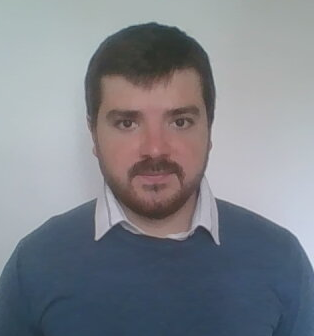
\includegraphics[width=\textwidth]{img/image_CV.png}
    \end{minipage}
\end{minipage}


\begin{minipage}[t]{0.28\textwidth}
    \begin{mdframed}[style=cadreCompetences]
        \section{Logiciel}
        \subsection{Dessin Technique}
        \begin{itemize}
            \item{Solidworks
                    \hfill
                    
\includegraphics[scale=0.25]{img/star.png} \hspace{-0.22cm}
                    
\includegraphics[scale=0.25]{img/star.png} \hspace{-0.22cm}
                    
\includegraphics[scale=0.25]{img/star.png} \hspace{-0.22cm}
                    
\includegraphics[scale=0.25]{img/star.png} \hspace{-0.22cm}
                    
\includegraphics[scale=0.25]{img/half_star.png}}
            \item{UG NX
                    \hfill
                    
\includegraphics[scale=0.25]{img/star.png} \hspace{-0.22cm}
                    
\includegraphics[scale=0.25]{img/star.png} \hspace{-0.22cm}
                    
\includegraphics[scale=0.25]{img/star.png} \hspace{-0.22cm}
                    
\includegraphics[scale=0.25]{img/star.png} \hspace{-0.22cm}
                    
\includegraphics[scale=0.25]{img/empty_star.png}}
            \item{Autocad
                    \hfill
                    
\includegraphics[scale=0.25]{img/star.png} \hspace{-0.22cm}
                    
\includegraphics[scale=0.25]{img/star.png} \hspace{-0.22cm}
                    
\includegraphics[scale=0.25]{img/star.png} \hspace{-0.22cm}
                    
\includegraphics[scale=0.25]{img/star.png} \hspace{-0.22cm}
                    
\includegraphics[scale=0.25]{img/empty_star.png}}
            \item{Creo/Pro E
                    \hfill
                    
\includegraphics[scale=0.25]{img/star.png} \hspace{-0.22cm}
                    
\includegraphics[scale=0.25]{img/star.png} \hspace{-0.22cm}
                    
\includegraphics[scale=0.25]{img/star.png} \hspace{-0.22cm}
                    
\includegraphics[scale=0.25]{img/empty_star.png} \hspace{-0.22cm}
                    
\includegraphics[scale=0.25]{img/empty_star.png}}
        \end{itemize}

        \subsection{Calcul numérique}
            \begin{itemize}
                \item{Solidworks
                    \hfill
                    
\includegraphics[scale=0.25]{img/star.png} \hspace{-0.22cm}
                    
\includegraphics[scale=0.25]{img/star.png} \hspace{-0.22cm}
                    
\includegraphics[scale=0.25]{img/star.png} \hspace{-0.22cm}
                    
\includegraphics[scale=0.25]{img/star.png} \hspace{-0.22cm}
                    
\includegraphics[scale=0.25]{img/empty_star.png}}
                \item{UG NX
                    \hfill
                    
\includegraphics[scale=0.25]{img/star.png} \hspace{-0.22cm}
                    
\includegraphics[scale=0.25]{img/star.png} \hspace{-0.22cm}
                    
\includegraphics[scale=0.25]{img/star.png} \hspace{-0.22cm}
                    
\includegraphics[scale=0.25]{img/star.png} \hspace{-0.22cm}
                    
\includegraphics[scale=0.25]{img/empty_star.png}}
                \item{Matlab
                    \hfill
                    
\includegraphics[scale=0.25]{img/star.png} \hspace{-0.22cm}
                    
\includegraphics[scale=0.25]{img/star.png} \hspace{-0.22cm}
                    
\includegraphics[scale=0.25]{img/star.png} \hspace{-0.22cm}
                    
\includegraphics[scale=0.25]{img/half_star.png} \hspace{-0.22cm}
                    
\includegraphics[scale=0.25]{img/empty_star.png}}
            \end{itemize}
        \subsection{Bureautique}
            \begin{itemize}
                \item{Excel
                    \hfill
                    
\includegraphics[scale=0.25]{img/star.png} \hspace{-0.22cm}
                    
\includegraphics[scale=0.25]{img/star.png} \hspace{-0.22cm}
                    
\includegraphics[scale=0.25]{img/star.png} \hspace{-0.22cm}
                    
\includegraphics[scale=0.25]{img/star.png} \hspace{-0.22cm}
                    
\includegraphics[scale=0.25]{img/half_star.png}}
                \item{Suite office
                    \hfill
                    
\includegraphics[scale=0.25]{img/star.png} \hspace{-0.22cm}
                    
\includegraphics[scale=0.25]{img/star.png} \hspace{-0.22cm}
                    
\includegraphics[scale=0.25]{img/star.png} \hspace{-0.22cm}
                    
\includegraphics[scale=0.25]{img/star.png} \hspace{-0.22cm}
                    
\includegraphics[scale=0.25]{img/empty_star.png}}
                \item{Latex
                    \hfill
                    
\includegraphics[scale=0.25]{img/star.png} \hspace{-0.22cm}
                    
\includegraphics[scale=0.25]{img/star.png} \hspace{-0.22cm}
                    
\includegraphics[scale=0.25]{img/star.png} \hspace{-0.22cm}
                    
\includegraphics[scale=0.25]{img/half_star.png} \hspace{-0.22cm}
                    \includegraphics[scale=0.25]{img/empty_star.png}}
            \end{itemize}

        \section{Programmation}
        \subsection{Applications}
            \begin{itemize}
                \item{VBA
                    \hfill
                    \includegraphics[scale=0.25]{img/star.png} \hspace{-0.22cm}
                    \includegraphics[scale=0.25]{img/star.png} \hspace{-0.22cm}
                    \includegraphics[scale=0.25]{img/star.png} \hspace{-0.22cm}
                    \includegraphics[scale=0.25]{img/star.png} \hspace{-0.22cm}
                    \includegraphics[scale=0.25]{img/star.png}}
                \item{Solidworks
                    \hfill
                    \includegraphics[scale=0.25]{img/star.png} \hspace{-0.22cm}
                    \includegraphics[scale=0.25]{img/star.png} \hspace{-0.22cm}
                    \includegraphics[scale=0.25]{img/star.png} \hspace{-0.22cm}
                    \includegraphics[scale=0.25]{img/star.png} \hspace{-0.22cm}
                    \includegraphics[scale=0.25]{img/empty_star.png}}
                \item{Langage C
                    \hfill
                    \includegraphics[scale=0.25]{img/star.png} \hspace{-0.22cm}
                    \includegraphics[scale=0.25]{img/star.png} \hspace{-0.22cm}
                    \includegraphics[scale=0.25]{img/star.png} \hspace{-0.22cm}
                    \includegraphics[scale=0.25]{img/half_star.png} \hspace{-0.22cm}
                    \includegraphics[scale=0.25]{img/empty_star.png}}
            \end{itemize}
        \subsection{Développement Web}
            \begin{itemize}
                \item{HTML/CSS
                    \hfill
                    \includegraphics[scale=0.25]{img/star.png} \hspace{-0.22cm}
                    \includegraphics[scale=0.25]{img/star.png} \hspace{-0.22cm}
                    \includegraphics[scale=0.25]{img/half_star.png} \hspace{-0.22cm}
                    \includegraphics[scale=0.25]{img/empty_star.png} \hspace{-0.22cm}
                    \includegraphics[scale=0.25]{img/empty_star.png}}
                \item{PHP
                    \hfill
                    \includegraphics[scale=0.25]{img/star.png} \hspace{-0.22cm}
                    \includegraphics[scale=0.25]{img/star.png} \hspace{-0.22cm}
                    \includegraphics[scale=0.25]{img/half_star.png} \hspace{-0.22cm}
                    \includegraphics[scale=0.25]{img/empty_star.png} \hspace{-0.22cm}
                    \includegraphics[scale=0.25]{img/empty_star.png}}
            \end{itemize}

        \section{Langues}
        \subsection{Anglais : C1 \newline (855 - Toeic 2015)}
            \begin{itemize}
                \item{Compréhension
                    \hfill
                    \includegraphics[scale=0.25]{img/star.png} \hspace{-0.22cm}
                    \includegraphics[scale=0.25]{img/star.png} \hspace{-0.22cm}
                    \includegraphics[scale=0.25]{img/star.png} \hspace{-0.22cm}
                    \includegraphics[scale=0.25]{img/star.png} \hspace{-0.22cm}
                    \includegraphics[scale=0.25]{img/half_star.png}}
                \item{Expression
                    \hfill
                    \includegraphics[scale=0.25]{img/star.png} \hspace{-0.22cm}
                    \includegraphics[scale=0.25]{img/star.png} \hspace{-0.22cm}
                    \includegraphics[scale=0.25]{img/star.png} \hspace{-0.22cm}
                    \includegraphics[scale=0.25]{img/half_star.png} \hspace{-0.22cm}
                    \includegraphics[scale=0.25]{img/empty_star.png}}
            \end{itemize}
        \subsection{Allemand : C1 \newline (881 - WIDAF 2015)}
            \begin{itemize}
                \item{Compréhension
                    \hfill
                    \includegraphics[scale=0.25]{img/star.png} \hspace{-0.22cm}
                    \includegraphics[scale=0.25]{img/star.png} \hspace{-0.22cm}
                    \includegraphics[scale=0.25]{img/star.png} \hspace{-0.22cm}
                    \includegraphics[scale=0.25]{img/half_star.png} \hspace{-0.22cm}
                    \includegraphics[scale=0.25]{img/empty_star.png}}
                \item{Expression
                    \hfill
                    \includegraphics[scale=0.25]{img/star.png} \hspace{-0.22cm}
                    \includegraphics[scale=0.25]{img/star.png} \hspace{-0.22cm}
                    \includegraphics[scale=0.25]{img/star.png} \hspace{-0.22cm}
                    \includegraphics[scale=0.25]{img/empty_star.png} \hspace{-0.22cm}
                    \includegraphics[scale=0.25]{img/empty_star.png}}
            \end{itemize}

        \section{Loisirs}
            \begin{itemize}
                \item{squash, vélotourisme}
                \item{série tv, lecture}
                \item{robotique, développement web}
            \end{itemize}
    \end{mdframed}
\end{minipage}
\hfill
\begin{minipage}[t]{0.68\textwidth}
    \vspace{0.15cm}
    \section{Formation}
        \begin{itemize}
            \item{2012--2016 : \textbf{Diplôme d'Ingénieur en Génie Mécanique} INSA Strasbourg (Anciennement ENSAIS)}
            \item{2010--2012 : Classe Préparatoire intégrée INSA Strasbourg \textbf{DeutschInsa} \newline (Moitié des enseignements en Allemand)}
            \item{Juin 2010 : Baccalauréat mention européenne Allemand -- mention \textbf{Bien}}
        \end{itemize}

    \section{Milton Roy : une entreprise, plusieurs expériences}
    \subsection{Juin 2018 -- Maintenant : Relais technique entre l'équipe agitation et le responsable Bureau d'Études}
    \begin{itemize}%
        \item{Partage du temps de travail entre le site de Samoreau (Bureau d'études agitation) et Pont-Saint-Pierre (Production)}
        \item{Maîtrise de Unigraphics NX et Autocad par apprentissage en autonomie}
        \item{Études agitateurs: Plans de détails et d'encombrement et gestion données ERP }
        \item{Déplacement en Inde pour définir les calculs mécaniques d'un outil de chiffrage.} 
        \item{Formation de l’équipe Indienne pour le développement d’un marché local}
    \end{itemize}

    \subsection{Juin 2017 -- Juin 2018 : Ingénieur études pompes doseuses}
    \begin{itemize}
        \item{Maîtrise de Solidworks par un apprentissage en autonomie.}
        \item{Études pompe: Plans de détails et d'encombrement et gestion données ERP }
        \item{Calculs: échange thermique (analytique), fréquences propres (Simulation), calcul contraintes (Simulation et analytique), ...}
        \item{Automatisation des plans d’encombrement par macro Solidworks (VBA)}
    \end{itemize}

    \subsection{Septembre 2016 -- Juin 2017 : Participation au transfert de production de Samoreau(77) à Pont-Saint-Pierre(27)}
    \begin{itemize}
        \item{Design des cuves et circuits hydrauliques des moyens d’essais pour agitateurs}
        \item{Développement d’outils d’analyse des données techniques de l’ERP pour tous les services (supply chain, documentation, production,...)}
        \item{Soutien technique pour l’adaptation des process et transfert des données techniques dans l’ERP (JD Edwards)}
        \item{Automatisation des nomenclatures (Excel) et plans d’encombrement (SVG)}
    \end{itemize}


    \subsection{2011 -- 2016 : Stages dans différents sites de l'entreprise}
    \begin{itemize}
        \item{Mars à Août 2016 -- Pont-Saint-Pierre (27) -- Rationalisation d’une gamme de doseurs}
        \item{Juin à Août 2015 -- Sunderland (Angleterre) -- Design d’un espace de test pour compresseurs}
        \item{Mars à Août 2014 -- Samoreau (77) -- Création de feuilles de calculs de dimensionnement d’agitateurs}
        \item{Juin à Août 2011 -- Samoreau (77) -- Mesures des propriétés hydrauliques d’hélices}
    \end{itemize}
\end{minipage}

\end{document}
